Having outlined a variety of models and metrics tracked for the
purposes of their objective comparison, we proceed to present and discuss our
results in the next sections.


\subsection{Results of Decoupled Sampling}
\label{sec:modelres}

We begin by comparing a diverse set of surrogate families that we proposed
to evaluate on previously collected samples of the expensive MC TBR model.
Through the four experimental cases described
in~\cref{sec:experiment-methodology}, we aim to study properties of the
considered models in terms of regression performance, training and prediction
time.

\subsubsection{Hyperparameter Tuning}

The first two experiments perform Bayesian optimisation to maximise~$R^2$ in
a cross-validation setting as a function of model hyperparameters. While in the
first experiment we limit training and test sets to the scope of four selected
slices of the feature space, in the second experiment we lift this restriction.

The results displayed in~\cref{fig:exp1-time-vs-reg} indicate that in the first
experiment, GBTs clearly appear to be the most accurate as
well as the fastest surrogate family in terms of mean prediction time. Following
that, we note that ERTs, SVMs and ANNs also achieved satisfactory results with respect to both examined metrics.
While the remainder of tested surrogate families does not exhibit problems in
complexity, its regression performance falls below average.

\begin{figure}[h]
	\centering
	\begin{subfigure}[b]{0.333\textwidth}
		\centering
		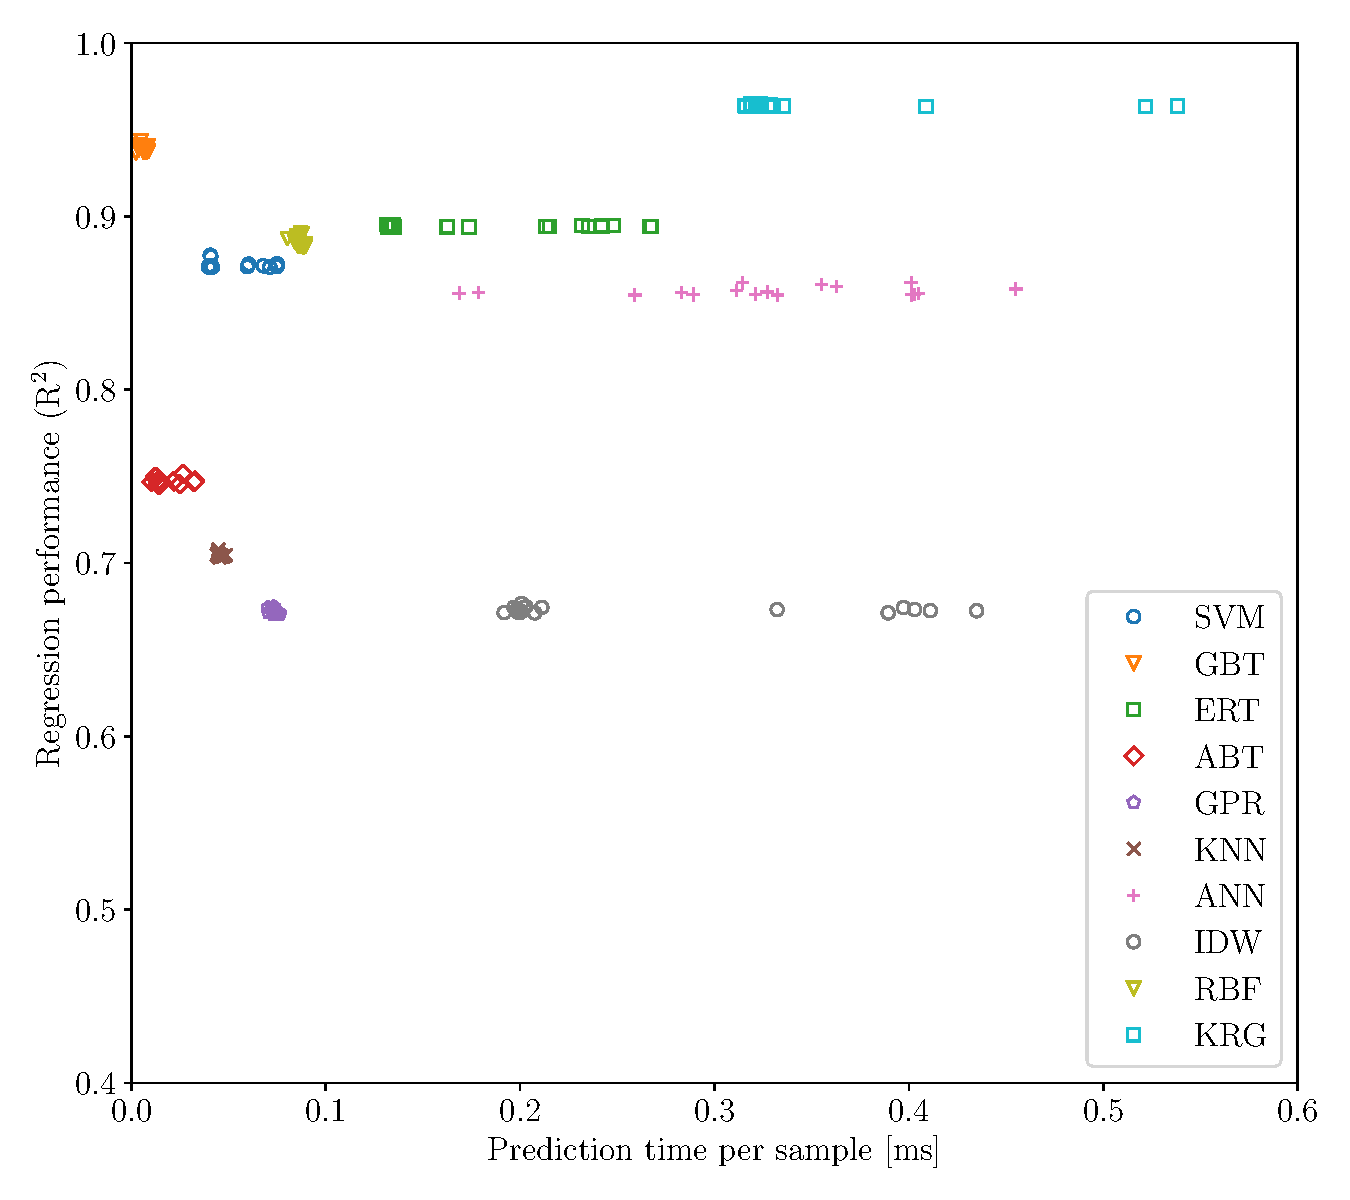
\includegraphics[width=\linewidth]{exp1_slice0}
		\caption{Run 2, batches 0-2}
	\end{subfigure}\hfill%
	\begin{subfigure}[b]{0.333\textwidth}
		\centering
		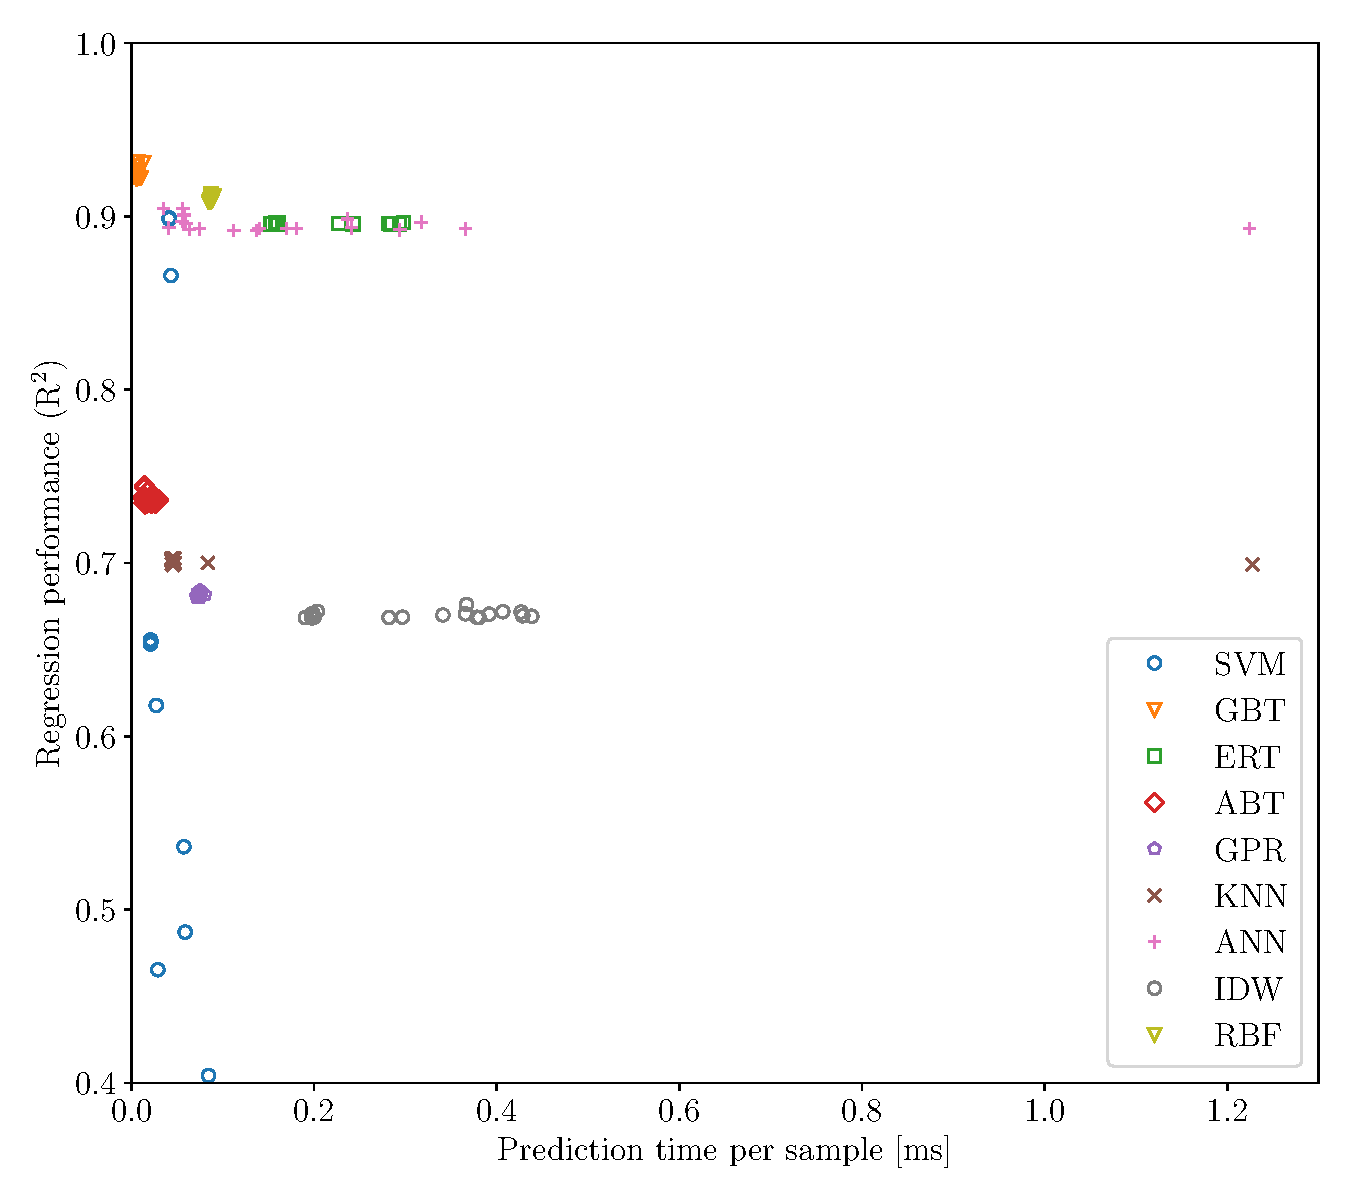
\includegraphics[width=\linewidth]{exp1_slice1}
		\caption{Run 2, batches 100-102}
	\end{subfigure}\hfill%
	\begin{subfigure}[b]{0.333\textwidth}
		\centering
		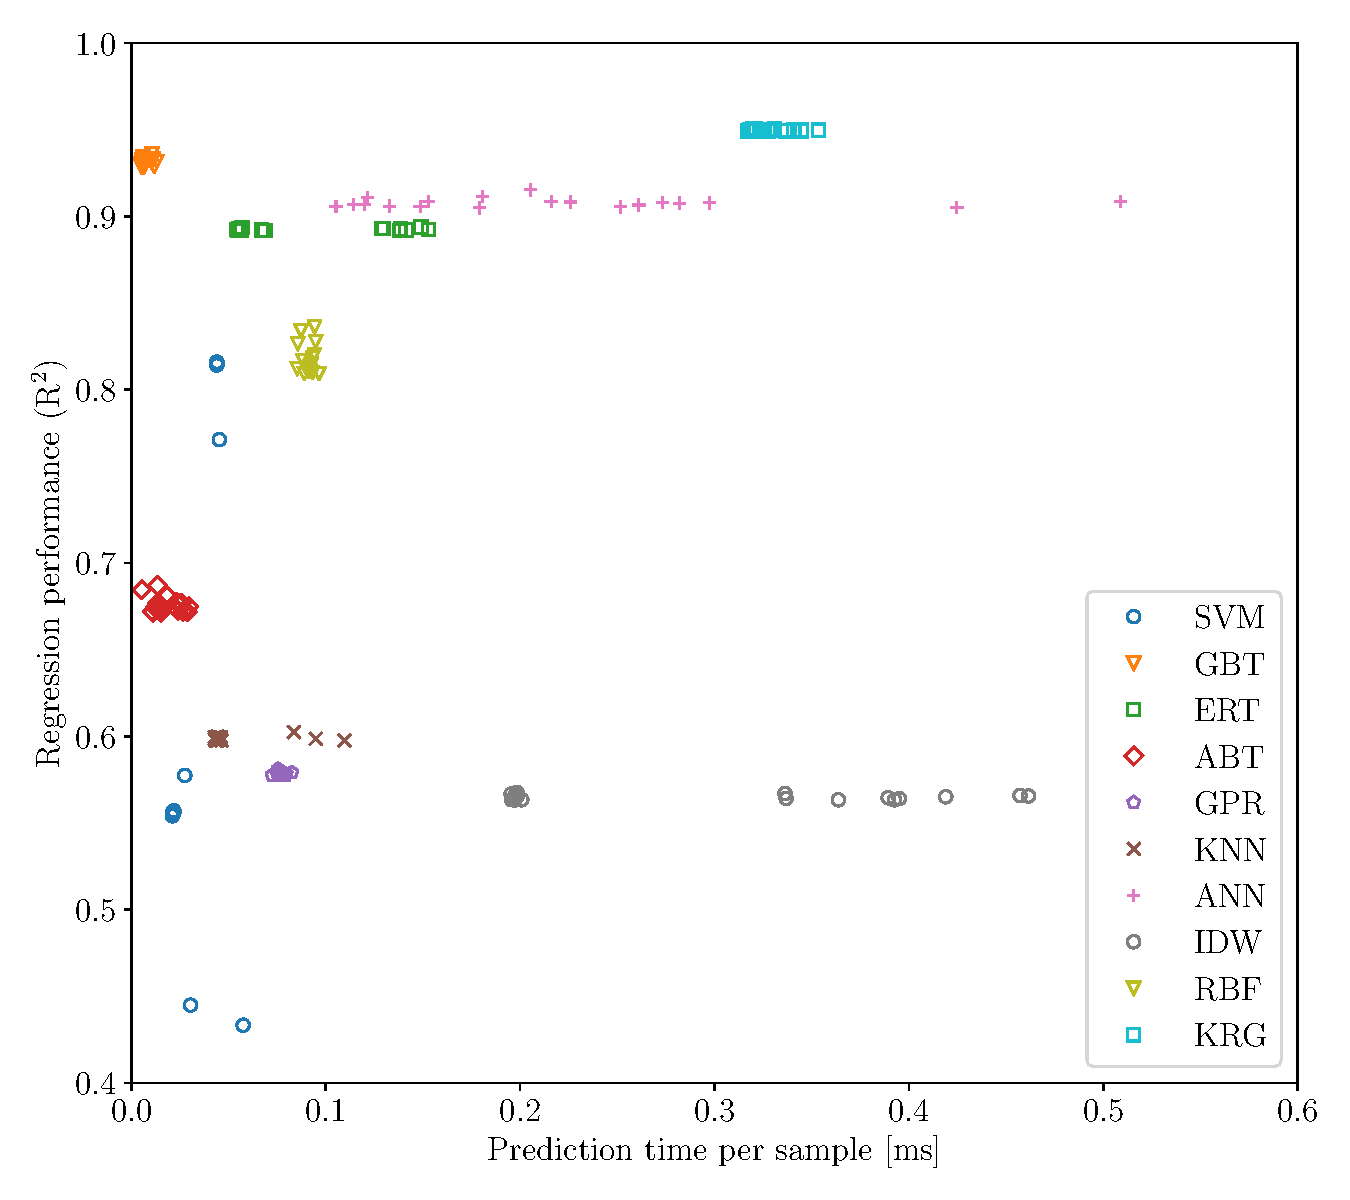
\includegraphics[width=\linewidth]{exp1_slice2}
		\caption{Run 2, batches 200-202}
	\end{subfigure}
	\caption{20~best-performing surrogates per each considered family, plotted in
		terms of complexity (as $\overline{t}_{\text{pred.}}$) and regression
		performance (as~$R^2$) on selected slices of run~2, evaluated in
	experiment~1. Here, batches refer to subsets of training and test datasets that
	may be matched to slices using~\cref{tbl:slices}.}
	\label{fig:exp1-time-vs-reg}
\end{figure}

\begin{wrapfigure}{r}{0.333\textwidth}
	\centering
	\vspace{-3ex}
	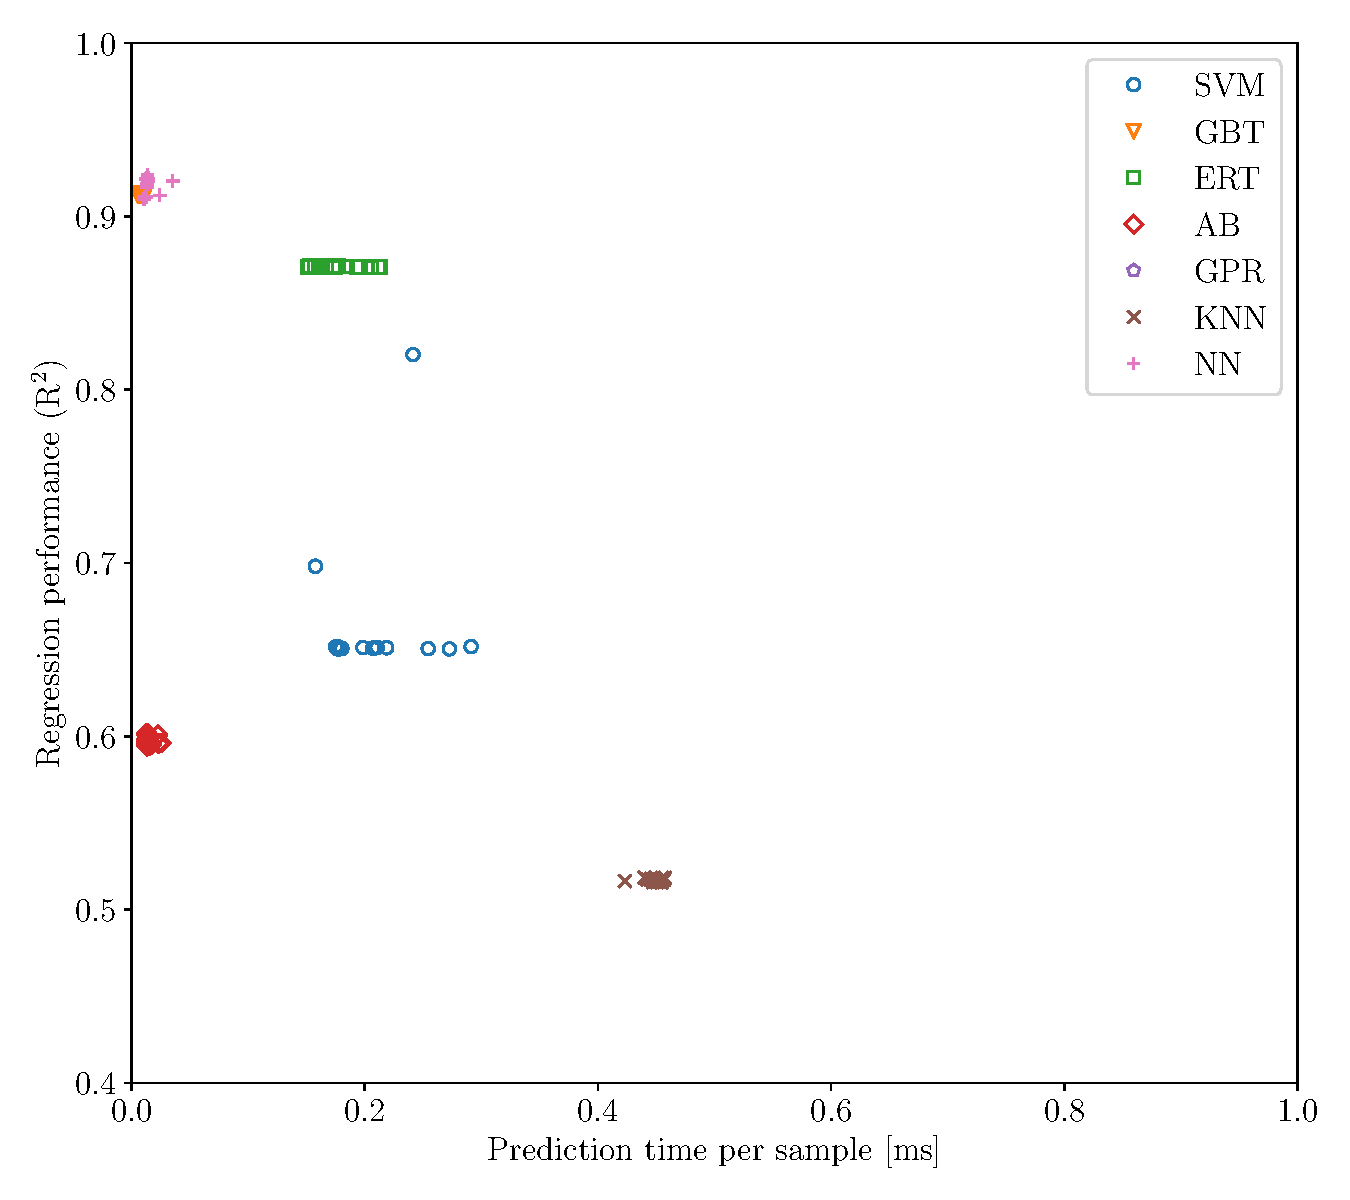
\includegraphics[width=\linewidth]{exp2_time_vs_reg}
	\caption{Results of experiment~2, plotted analogously
	to~\cref{fig:exp1-time-vs-reg}.}
	\label{fig:exp2-time-vs-reg}
	\vspace{-4ex}
\end{wrapfigure}

The results of the second experiment, shown in~\cref{fig:exp2-time-vs-reg},
seem to confirm our expectations. Compared to the previous case, we observe
that many surrogate families consistently achieved worse regression
performance and prediction times in a more complex, unrestricted domain. The least
affected models appear to be GBTs, ANNs and ERTs, which are known to be capable of capturing relationships
involving mixed feature types that were deliberately withheld in the first
experiment. With only negligible differences, the first two of these families
appear to be tied for the best performance as well as the shortest prediction
time. We observe that ERTs trees and RBFs also
demonstrated satisfactory results, outperforming the remaining surrogates in
terms of regression performance, and in some cases also in prediction time.

Following both hyperparameter tuning experiments, we conclude that while domain
restrictions employed in the first case have proven effective in improving the
regression performance of some methods, this result has fluctuated considerably
depending on the selected slices. Furthermore, in all instances the best
results were achieved by families of surrogates that were nearly unaffected by
this modification.


\subsubsection{Scaling Benchmark}

In the third experiment we examine surrogate scaling properties by correlating
metrics of interest with training set size. First, the results shown 
in~\cref{fig:scaling-r2} suggest that the most accurate families from the previous experiments
consistently maintain their relative advantage over others, even as we introduce
more training data. While such families achieve nearly comparable regression
performance on the largest dataset, in the opposite case methods based on
decision trees clearly outperform neural networks. This can be observed
particularly on training sets of sizes up to~\num{6000}.

\begin{figure}[h]
	\centering
	\begin{subfigure}[b]{0.333\textwidth}
		\centering
		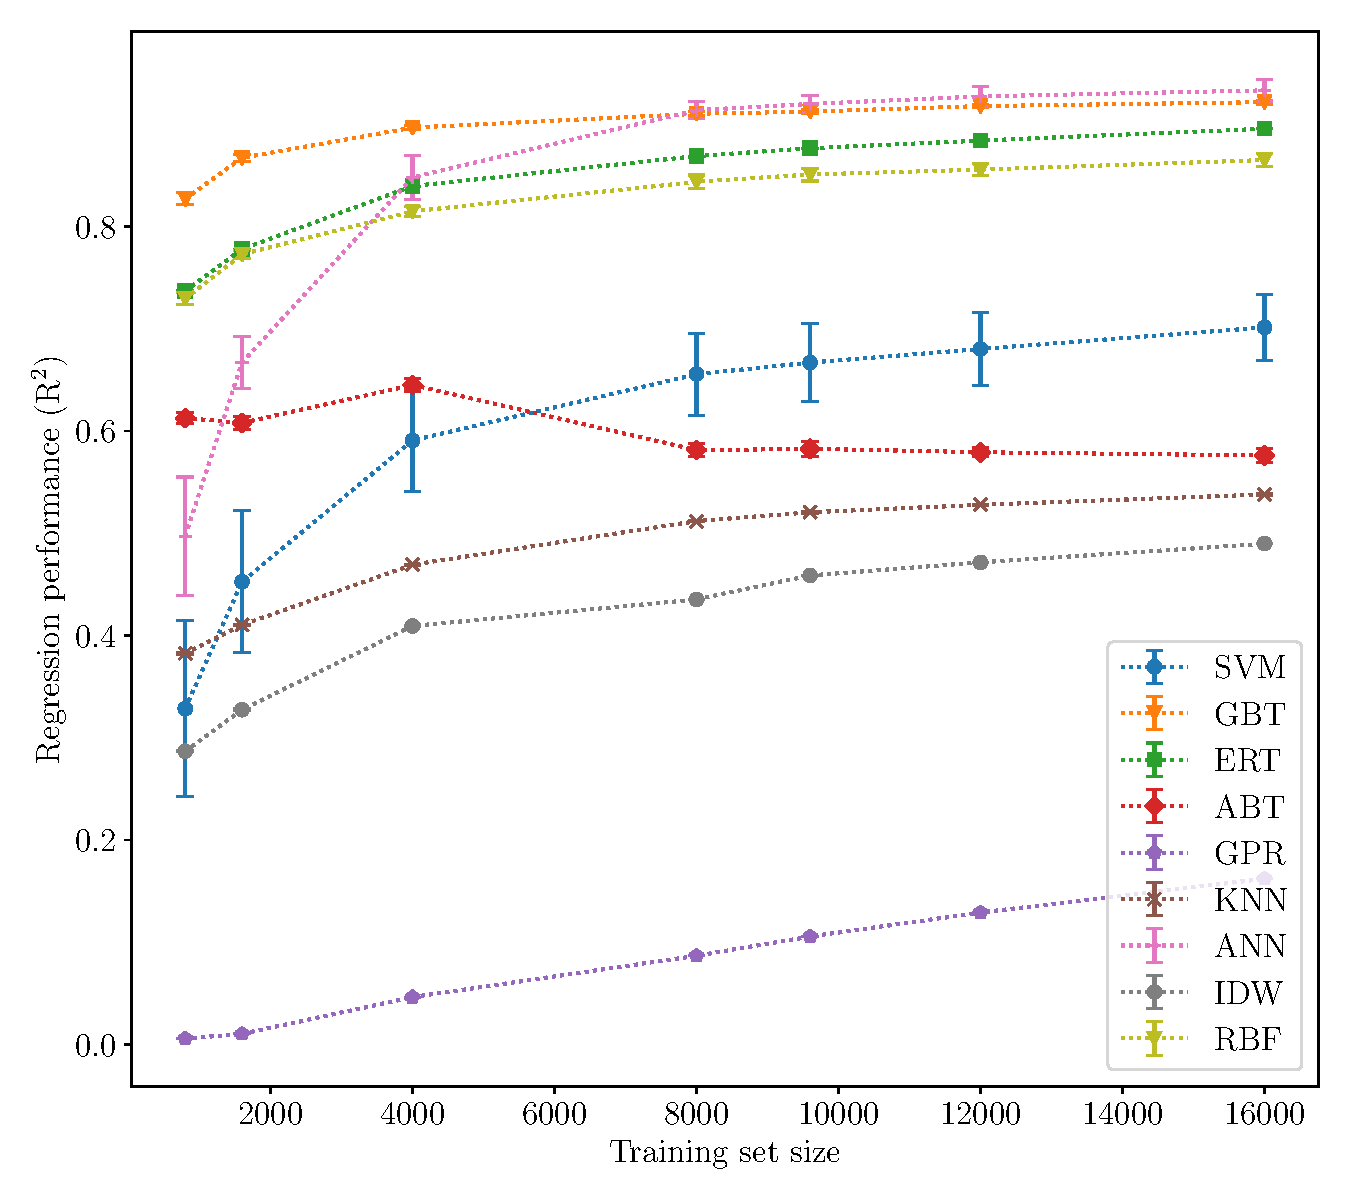
\includegraphics[width=\linewidth]{scaling_metric_r2}
		\caption{Regression performance (as $R^2$)}
		\label{fig:scaling-r2}
	\end{subfigure}\hfill%
	\begin{subfigure}[b]{0.333\textwidth}
		\centering
		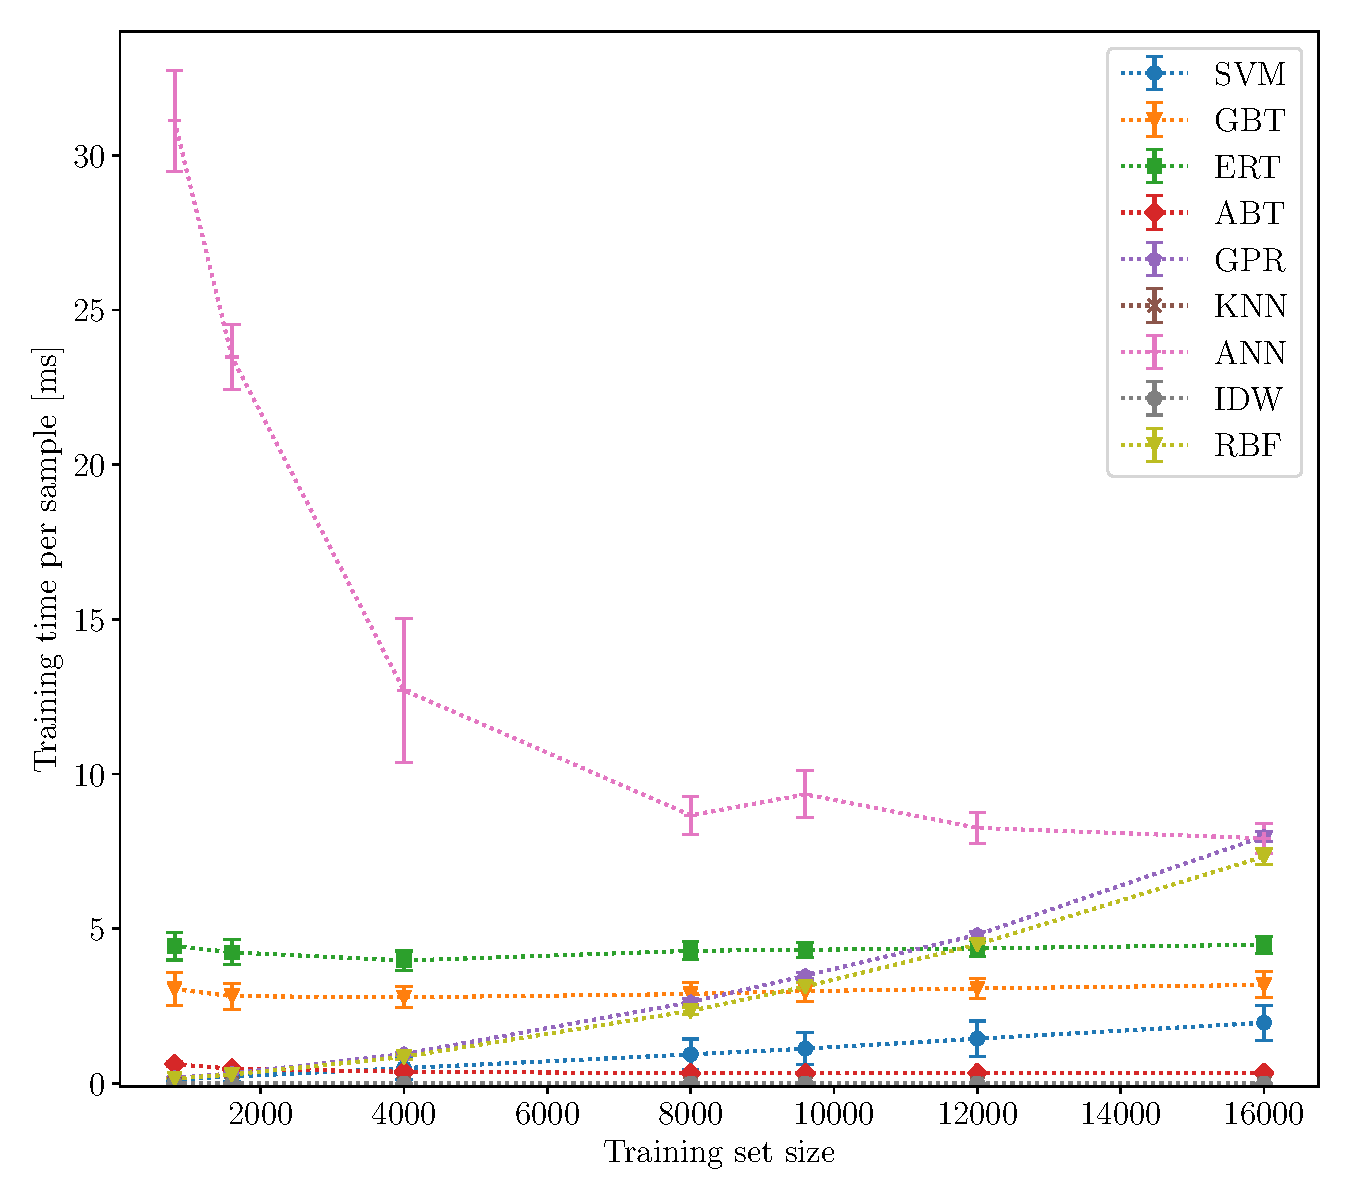
\includegraphics[width=\linewidth]{scaling_time_train}
		\caption{Complexity (as~$\overline{t}_{\text{trn.}}$)}
		\label{fig:scaling-trn}
	\end{subfigure}\hfill%
	\begin{subfigure}[b]{0.333\textwidth}
		\centering
		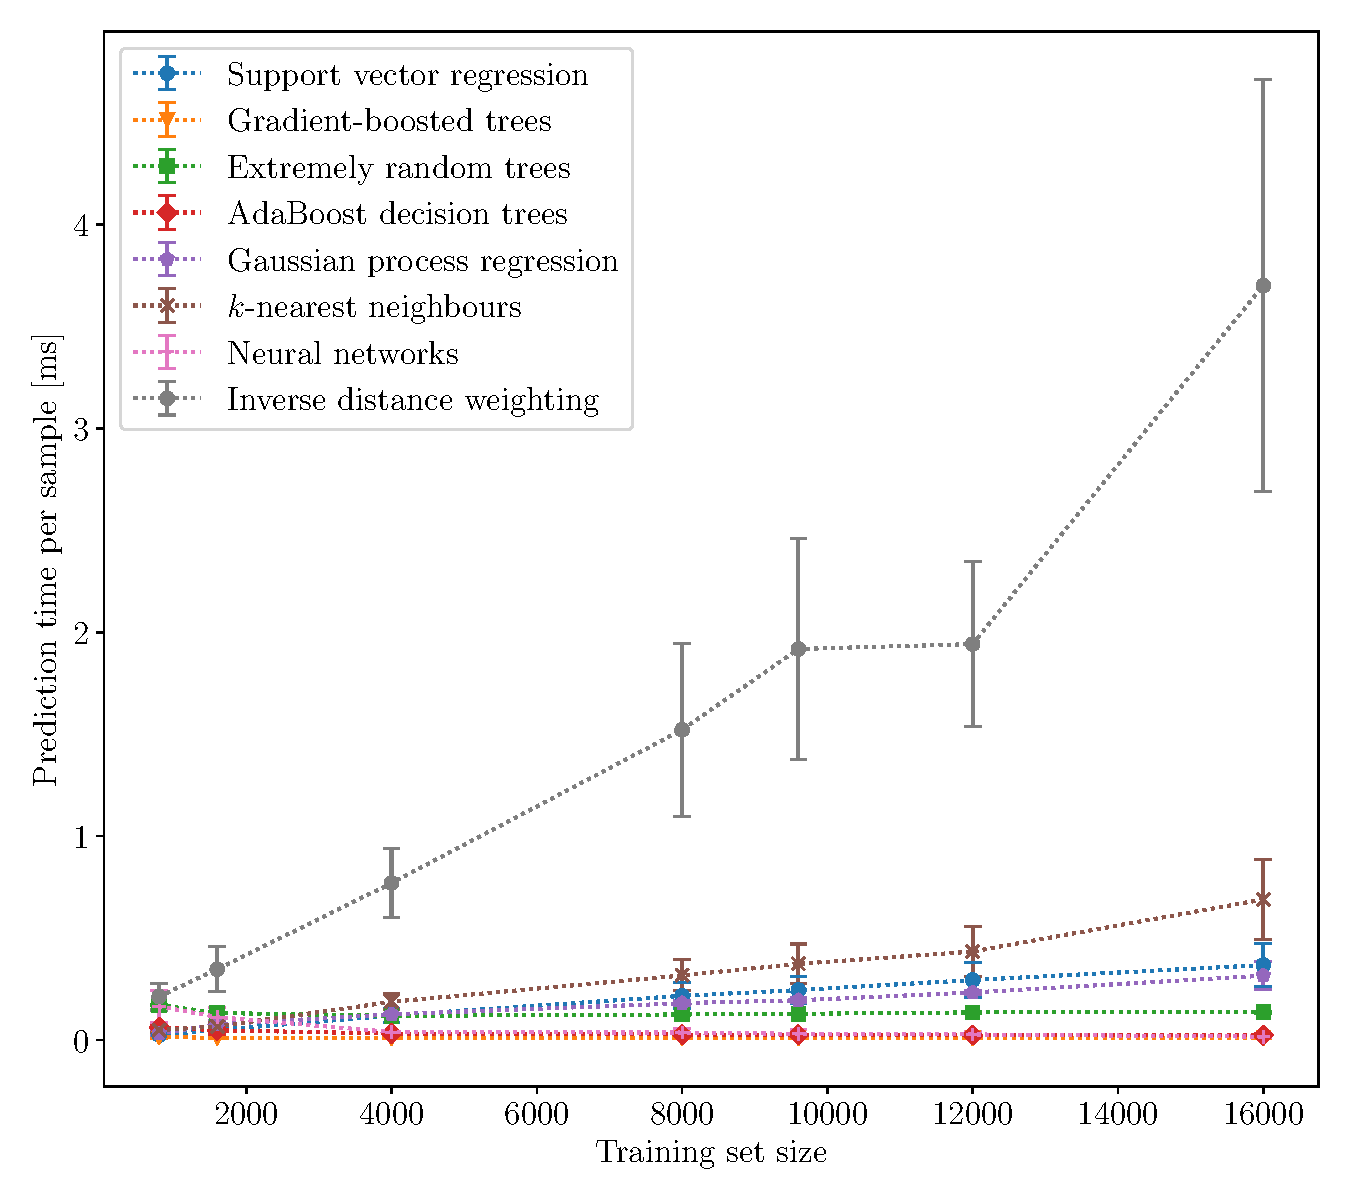
\includegraphics[width=\linewidth]{scaling_time_pred}
		\caption{Complexity (as~$\overline{t}_{\text{pred.}}$)}
		\label{fig:scaling-pred}
	\end{subfigure}
	\caption{Various metrics collected during experiment 3 (scaling
	benchmark) displayed as a function of training set size.}
	\label{fig:scaling}
\end{figure}

Next, we examine scaling behaviour in terms of the mean training time (displayed
in~\cref{fig:scaling-trn}). Consistent with our expectation, the shortest times
were achieved by instance-based learning methods (e.g. KNN, IDW) that
are trained trivially at the expense of increased lookup complexity later during prediction.
Furthermore, we observe that the majority of tree-based algorithms also exhibit
desirable properties unlike RBFs and gaussian process
regression, which appear to scale superlinearly. We note that ANNs,
which are the only family to utilise parallelisation during training, show an
inverse scaling characteristic. Our conjecture is that this effect may be caused
by a constant multi-threading overhead that possibly dominates the training process
on relatively small training sets.

Lastly, we study scaling with respect to the mean prediction time (shown
in~\cref{fig:scaling-pred}). Our initial observation is that all tested
surrogate families with the exception of previously mentioned instance-based
learning methods offer desirable characteristics overall. Analogous to previous
experiments, GBTs and ANNs again
appear to be tied, as they not only exhibit comparable times but also similar
scaling slopes.


\subsubsection{Model Comparison}

In the fourth and final experiment, we exploit previously collected information
to produce surrogates with desirable properties for practical use. We
aim to create models that yield: (i)~the best regression performance regardless
of other features, (ii)~acceptable performance with the shortest mean
prediction time, or (iii)~acceptable performance with the smallest training set.
To this end, we trained 8~surrogates that are presented in~\cref{fig:reg-performance}
(more details are given in~\cref{tbl:exp4-detailed-results} in the Appendix).

\begin{figure}[h]
	\centering
	\begin{subfigure}[b]{0.25\textwidth}
		\centering
		\includegraphics[width=\linewidth]{exp4_model1}
	\end{subfigure}\hfill%
	\begin{subfigure}[b]{0.25\textwidth}
		\centering
		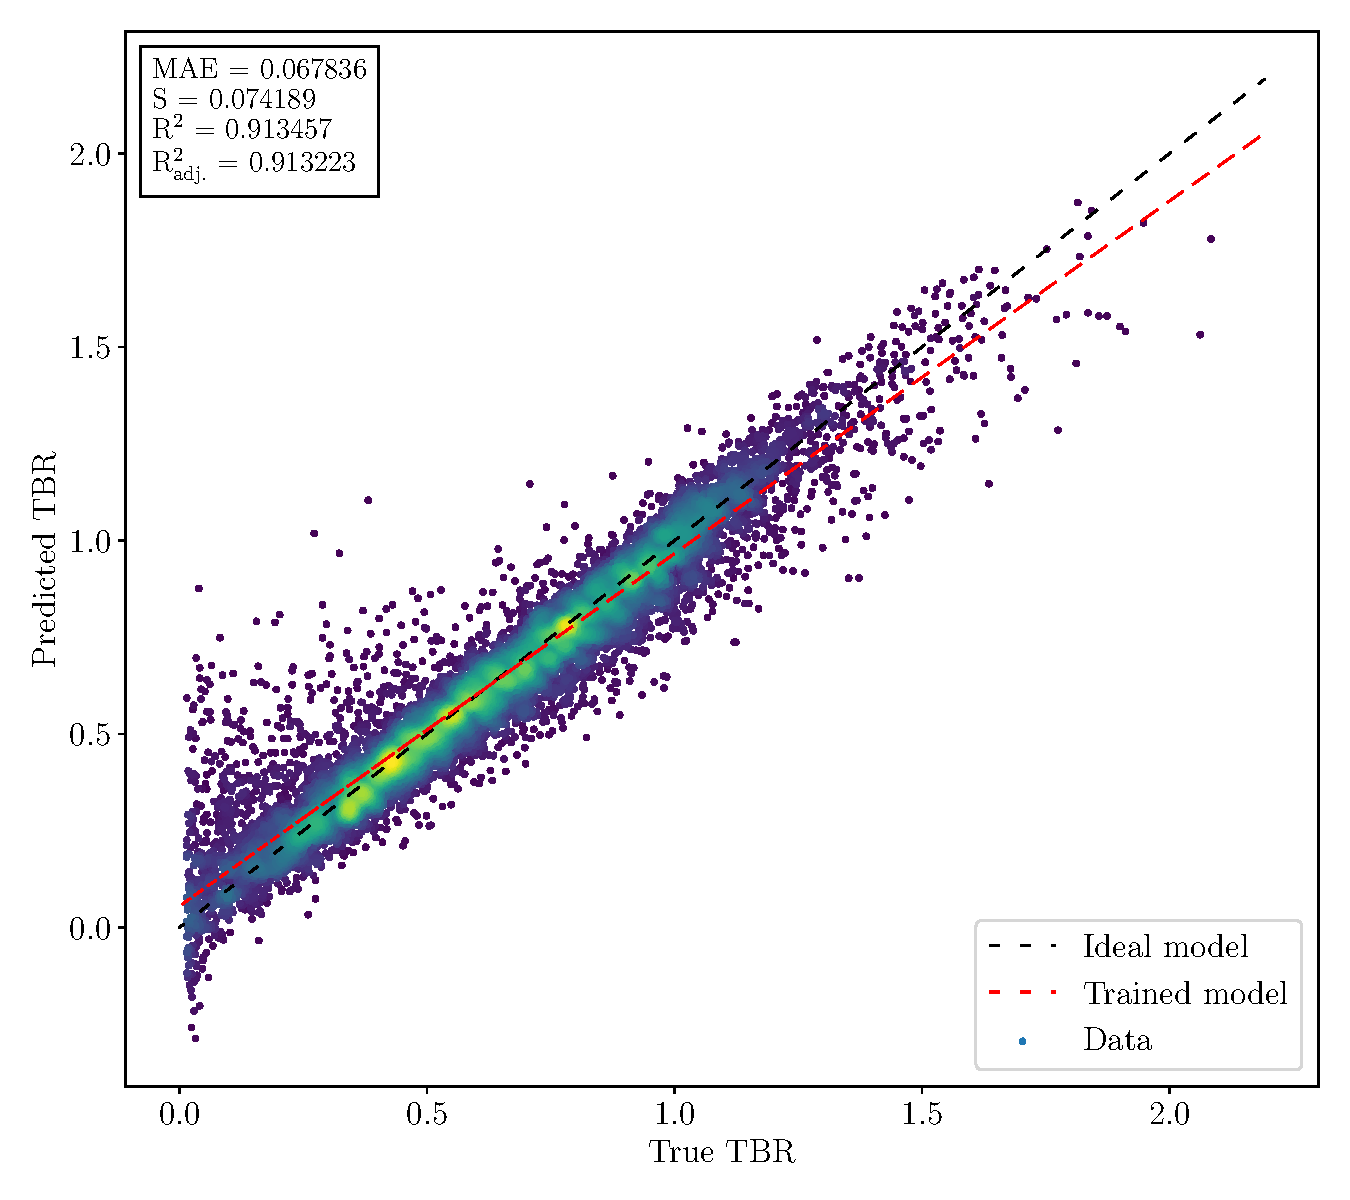
\includegraphics[width=\linewidth]{exp4_model2}
	\end{subfigure}\hfill%
	\begin{subfigure}[b]{0.25\textwidth}
		\centering
		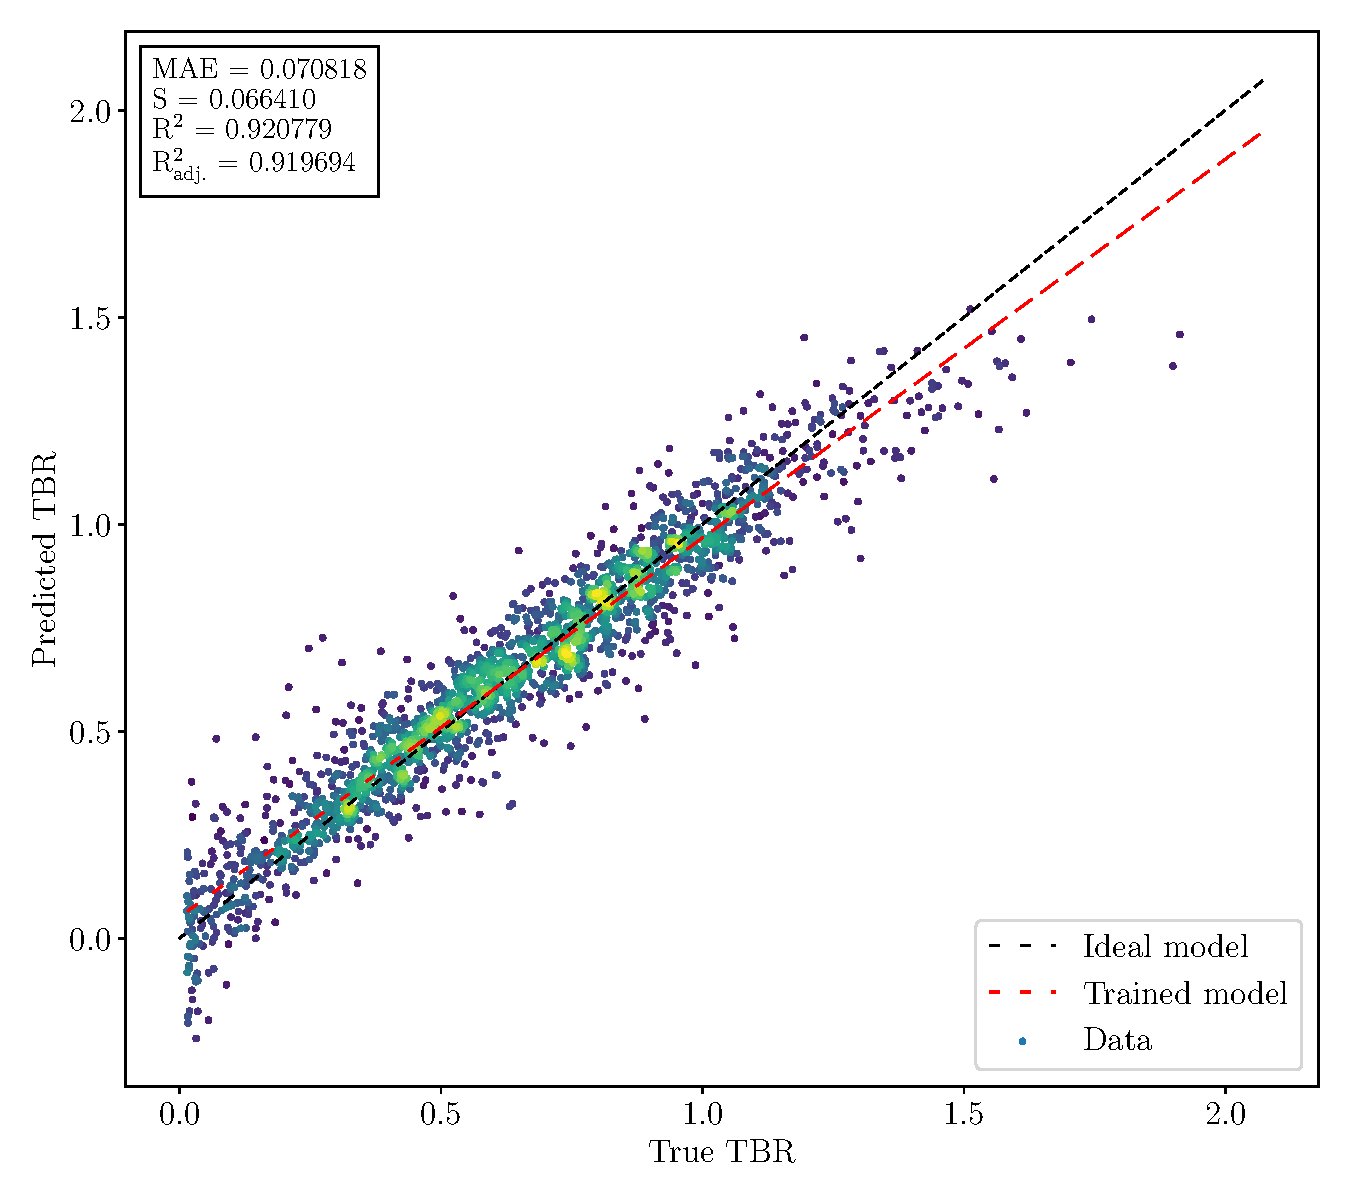
\includegraphics[width=\linewidth]{exp4_model3}
	\end{subfigure}\hfill%
	\begin{subfigure}[b]{0.25\textwidth}
		\centering
		\includegraphics[width=\linewidth]{exp4_model4}
	\end{subfigure}

	\begin{subfigure}[b]{0.25\textwidth}
		\centering
		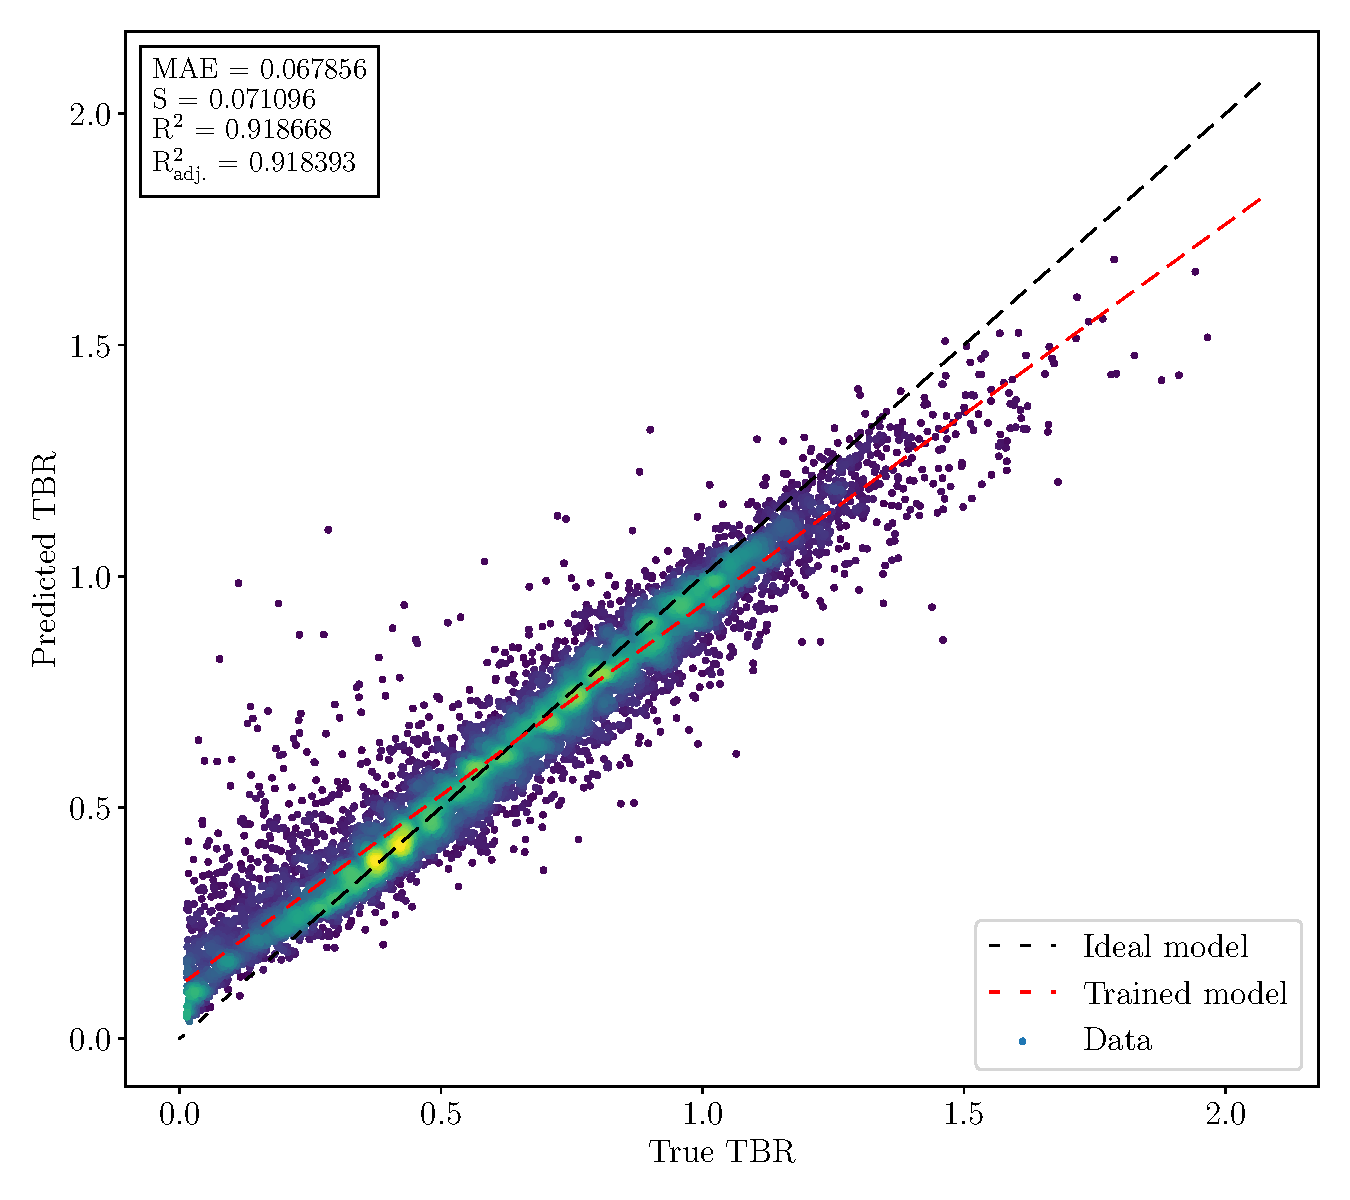
\includegraphics[width=\linewidth]{exp4_model5}
	\end{subfigure}\hfill%
	\begin{subfigure}[b]{0.25\textwidth}
		\centering
		\includegraphics[width=\linewidth]{exp4_model6}
	\end{subfigure}\hfill%
	\begin{subfigure}[b]{0.25\textwidth}
		\centering
		\includegraphics[width=\linewidth]{exp4_model7}
	\end{subfigure}\hfill%
	\begin{subfigure}[b]{0.25\textwidth}
		\centering
		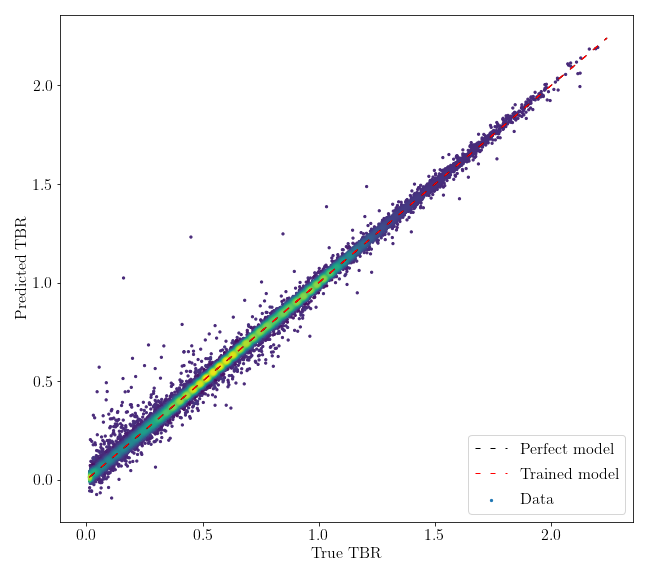
\includegraphics[width=\linewidth]{run1_5ke_1h3f128_4974_performance}
		% TODO: only a placeholder, regenerate when data becomes available
	\end{subfigure}
	\caption{Regression performance of models 1-4 (row 1, from the left) and 5-8
		(row 2) trained in experiment~4 (model comparison), viewed
		as true vs. predicted TBR on a test set of a selected cross-validation
		fold. Points are coloured by density.}
	\label{fig:reg-performance}
\end{figure}

Having selected ANNs, GBTs, ERTs, RBFs and SVMs based on the results of the
experiments~2-3, we utilised the best-performing hyperparameter
assignments and training sets of varying sizes. In attempts to satisfy
goals~(i) and~(ii) within cross-validation setting, our best surrogate
achieved~$R^2=\num{0.998}$ and mean prediction
time~$\overline{t}_{\text{pred.}}=\SI{0.898}{\micro\second}$. These correspond
to the standard error of regression~$S=\num{0.013}$ and a relative speedup~$\sigma=\num{8659251} \times$
with respect to the MC TBR evaluation baseline measured during run~1
(see~\cref{tbl:sampling-runs} for details). While this particular surrogate
used the entire available set of~\num{500000} datapoints, in attempts to satisfy
goal~(iii) we also learned a more simplified model that achieved~$R^2=\num{0.913}$,
$\overline{t}_{\text{pred.}}=\SI{6}{\micro\second}$, $S=\num{0.072}$ and $\sigma=\num{1269777} \times$
using only a set of size~\num{10000}.

Overall we found that due to their excellent performance, boosted tree-based
approaches seem to be advantageous for fast surrogate modelling on relatively small training
sets (up to the order of~$10^4$). Conversely, while neural networks perform
poorly in such a setting, both their regression performance and prediction times
have proven superior on larger training sets (at least of the order of~$10^5$).


\subsection{Results of Adaptive Sampling}
\label{sec:adaptiveres}

\begin{wrapfigure}{r}{0.4\textwidth}
  \vspace{-60pt}
  \begin{center}
    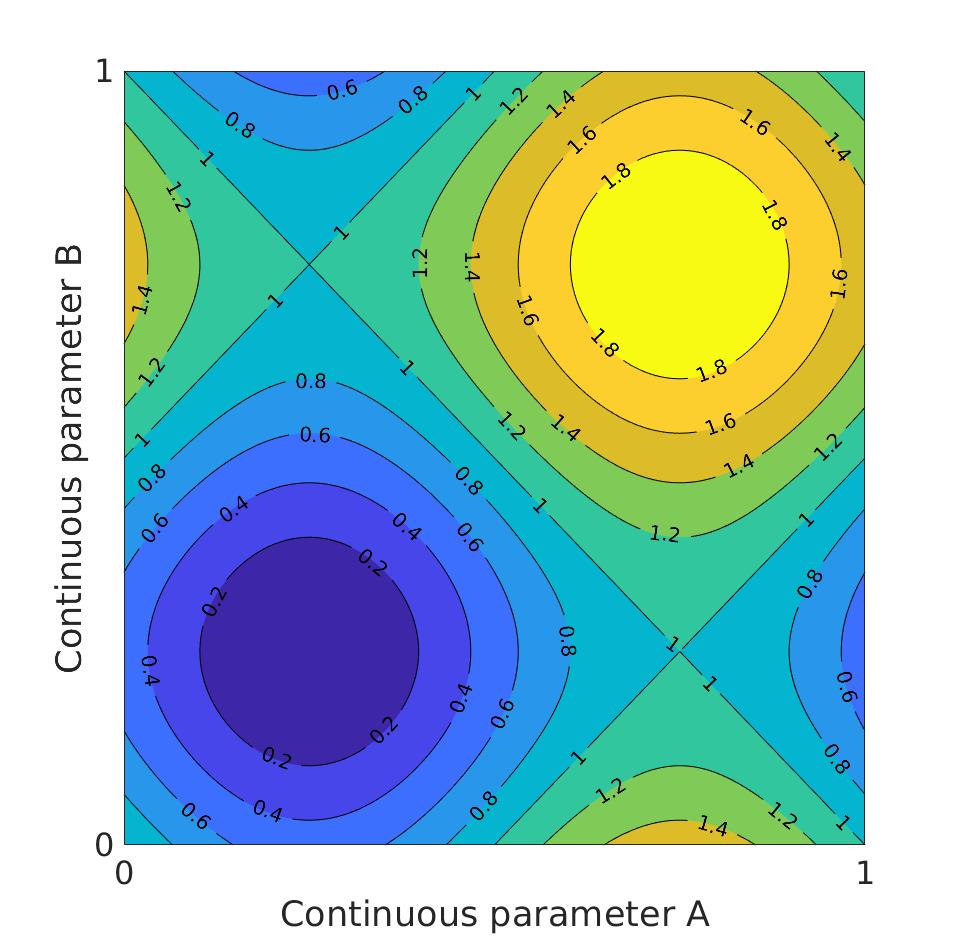
\includegraphics[width=0.4\textwidth]{fig5_sintoy.jpg}
	\caption{Sinusoidal toy TBR theory over two continuous parameters, wavenumber 1}
    \label{fig:sintoy}
  \end{center}
  \vspace{-10pt}
\end{wrapfigure}

In order to test our QASS prototype, several functional toy theories for TBR were developed as alternatives to the expensive MC model. By far the most robust of these was the following sinusoidal theory with adjustable wavenumber parameter $n$:

\begin{equation}
	\text{TBR} = \text{Mean}_{i \in C} \left[ \frac{1 + \sin(2\pi n (x_i - 1/2)) }{2} \right]
\end{equation}

plotted in~\cref{fig:sintoy} for $n=1$ and two continuous parameters $C$. ANNs
trained on this model demonstrated similar performance to those on the expensive
MC model. QASS performance was verified by training a $\text{1h3f}(256)$ ANN on
the sinusoidal theory for varied quantities of initial, incremental, and MCMC
candidate samples. Although the scope of this project did not include thorough
searches of this hyperparameter domain, sufficient runs were made to identify
some likely trends.

An increase in MCMC candidate samples was seen to have a positive but very weak
effect on final surrogate precision, suggesting that the runtime of MCMC on each
iteration can be limited for increased efficiency. -- Awaiting test results on
initial sample quantity --. The most complex dynamics arose with the adjustment
of sample increment, shown in~\cref{fig:qassincr}. For each tested initial sample quantity N, the optimal number of step samples was seen to be well-approximated by $\sqrt{N}$; the plotted error trends suggest that incremental samples larger than this optimum give slower model improvement on both the training and evaluation sets, and a larger minimum error on the evaluation set. This performance distinction is predicted to be even more significant when trained on the expensive MC model, where the number of sample evaluations will serve as the primary bottleneck for computation time.
\begin{figure}[h!]
    \centering
    \begin{subfigure}[t]{0.5\textwidth}
        \centering
        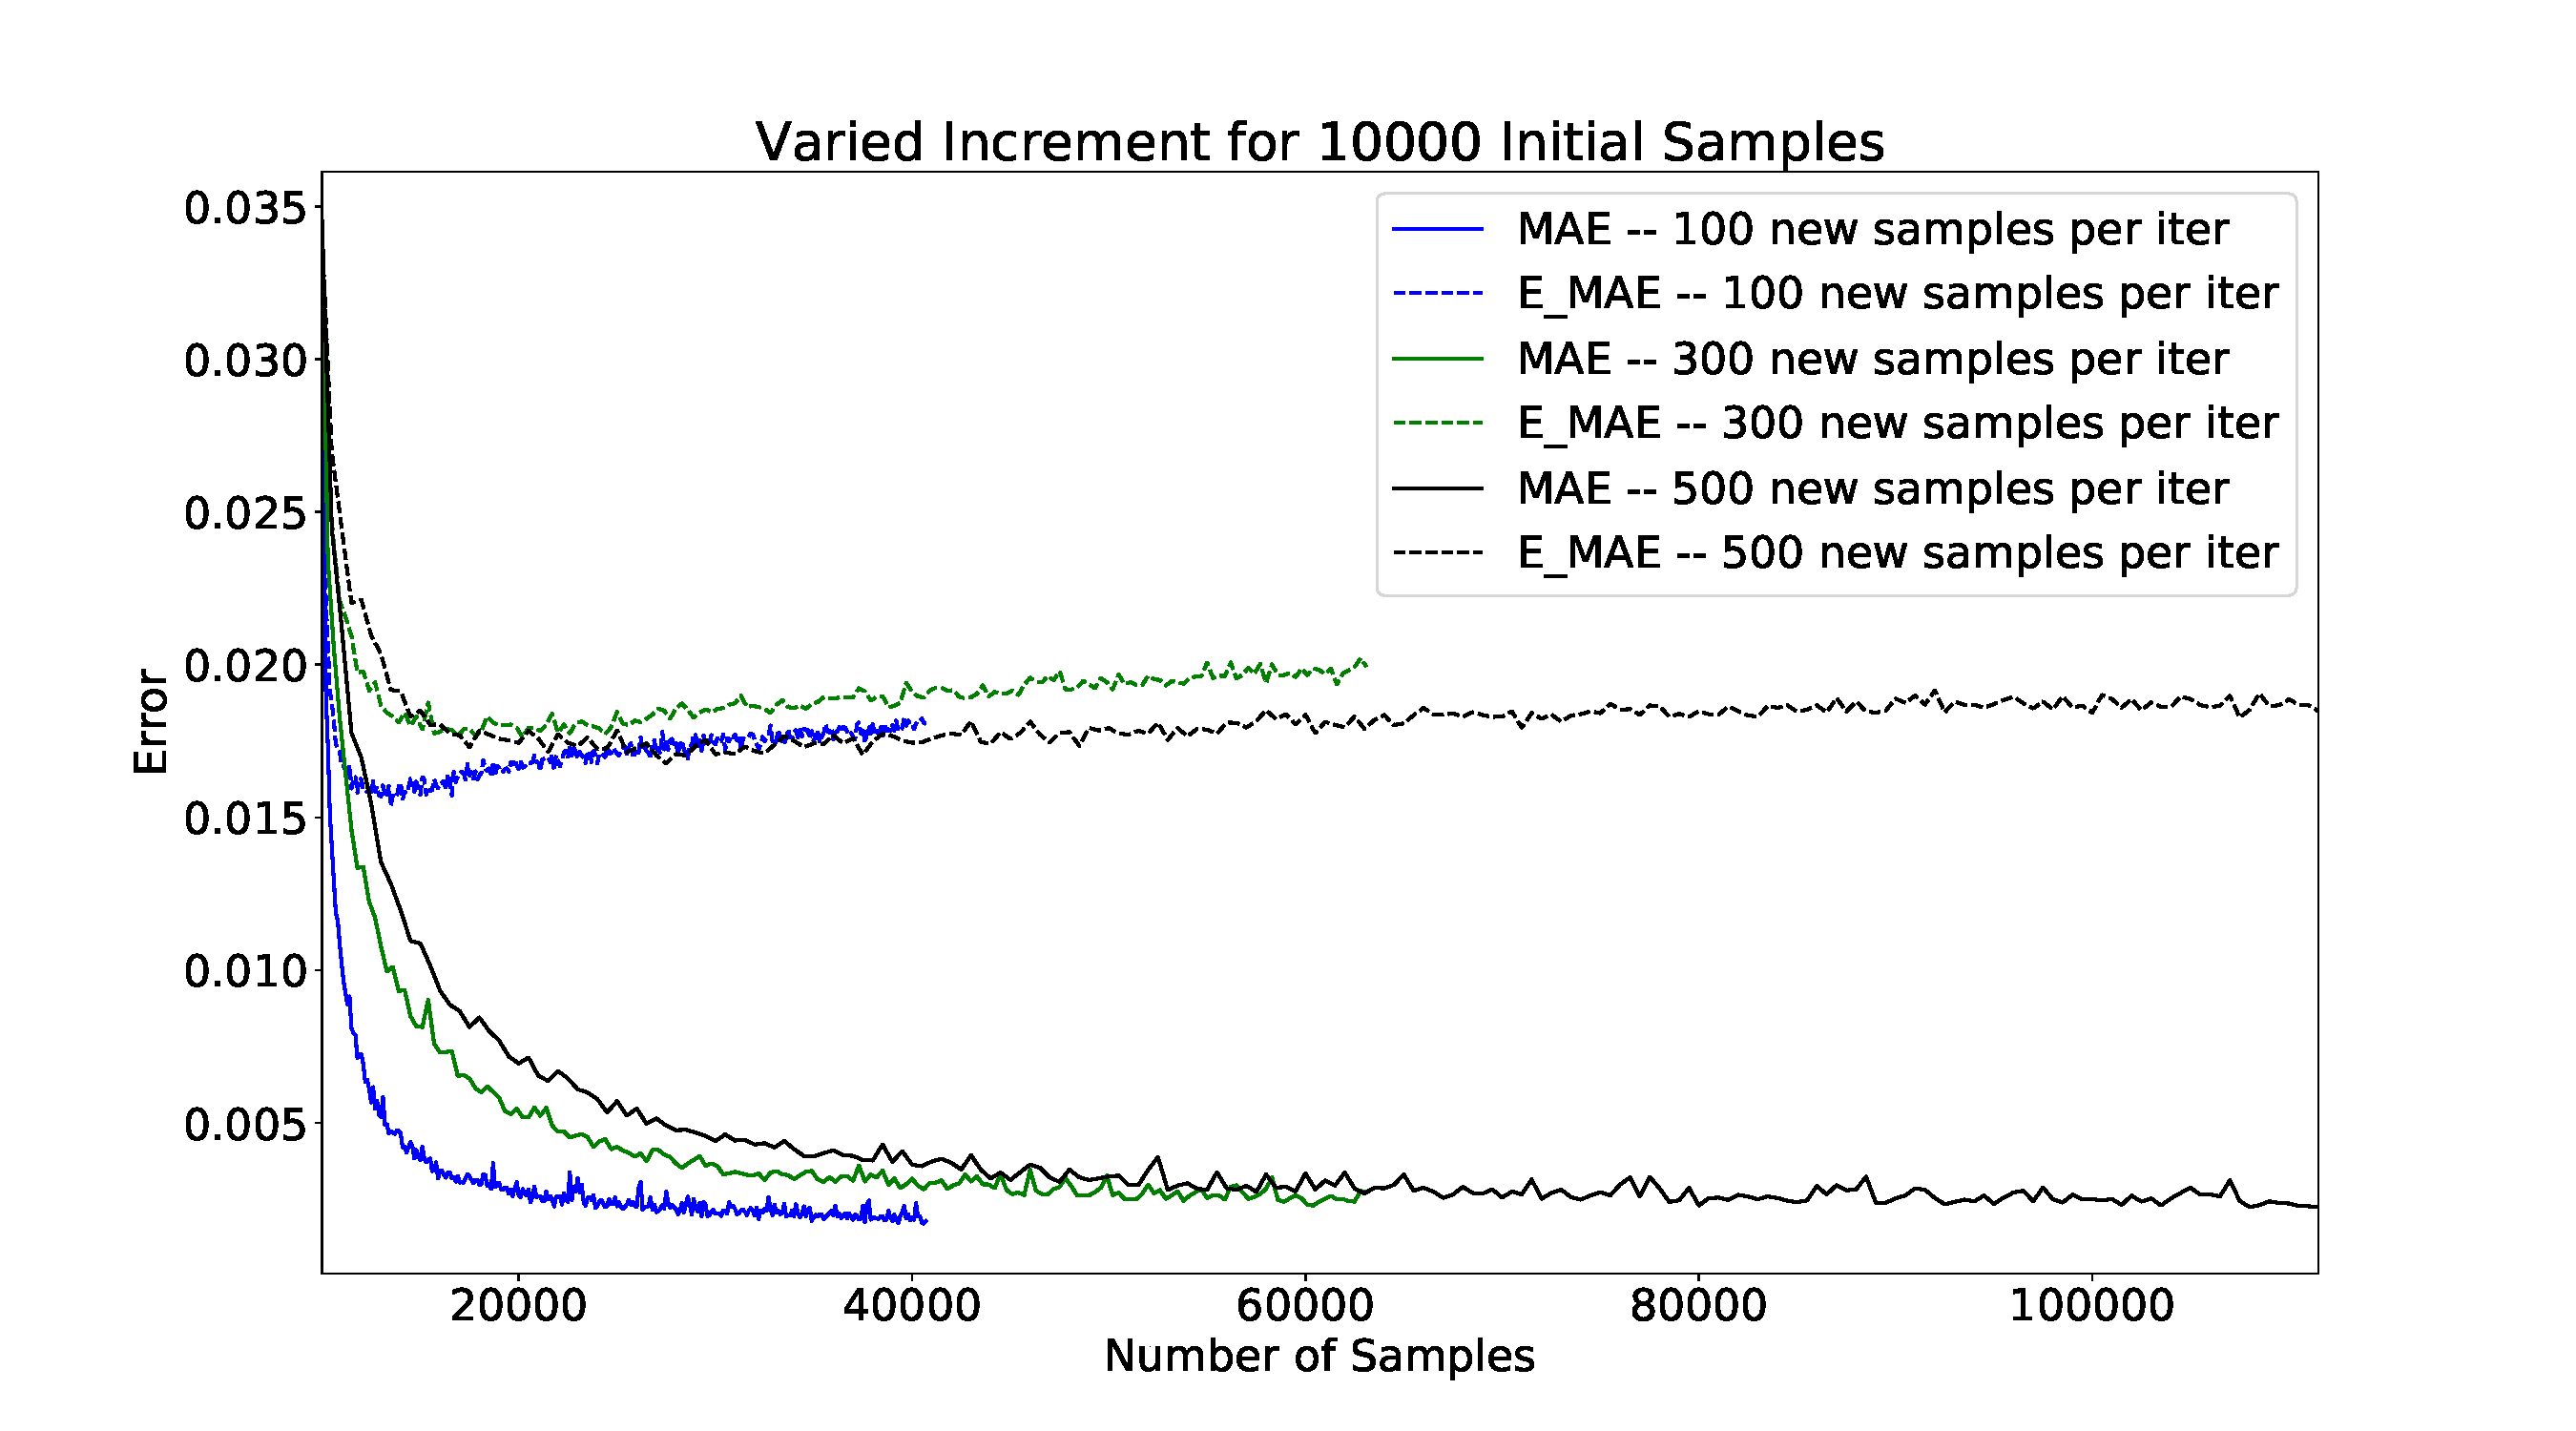
\includegraphics[width=1.1\linewidth]{fig6a_qassincrsamp.pdf}
    \end{subfigure}%
    ~ 
    \begin{subfigure}[t]{0.5\textwidth}
        \centering
        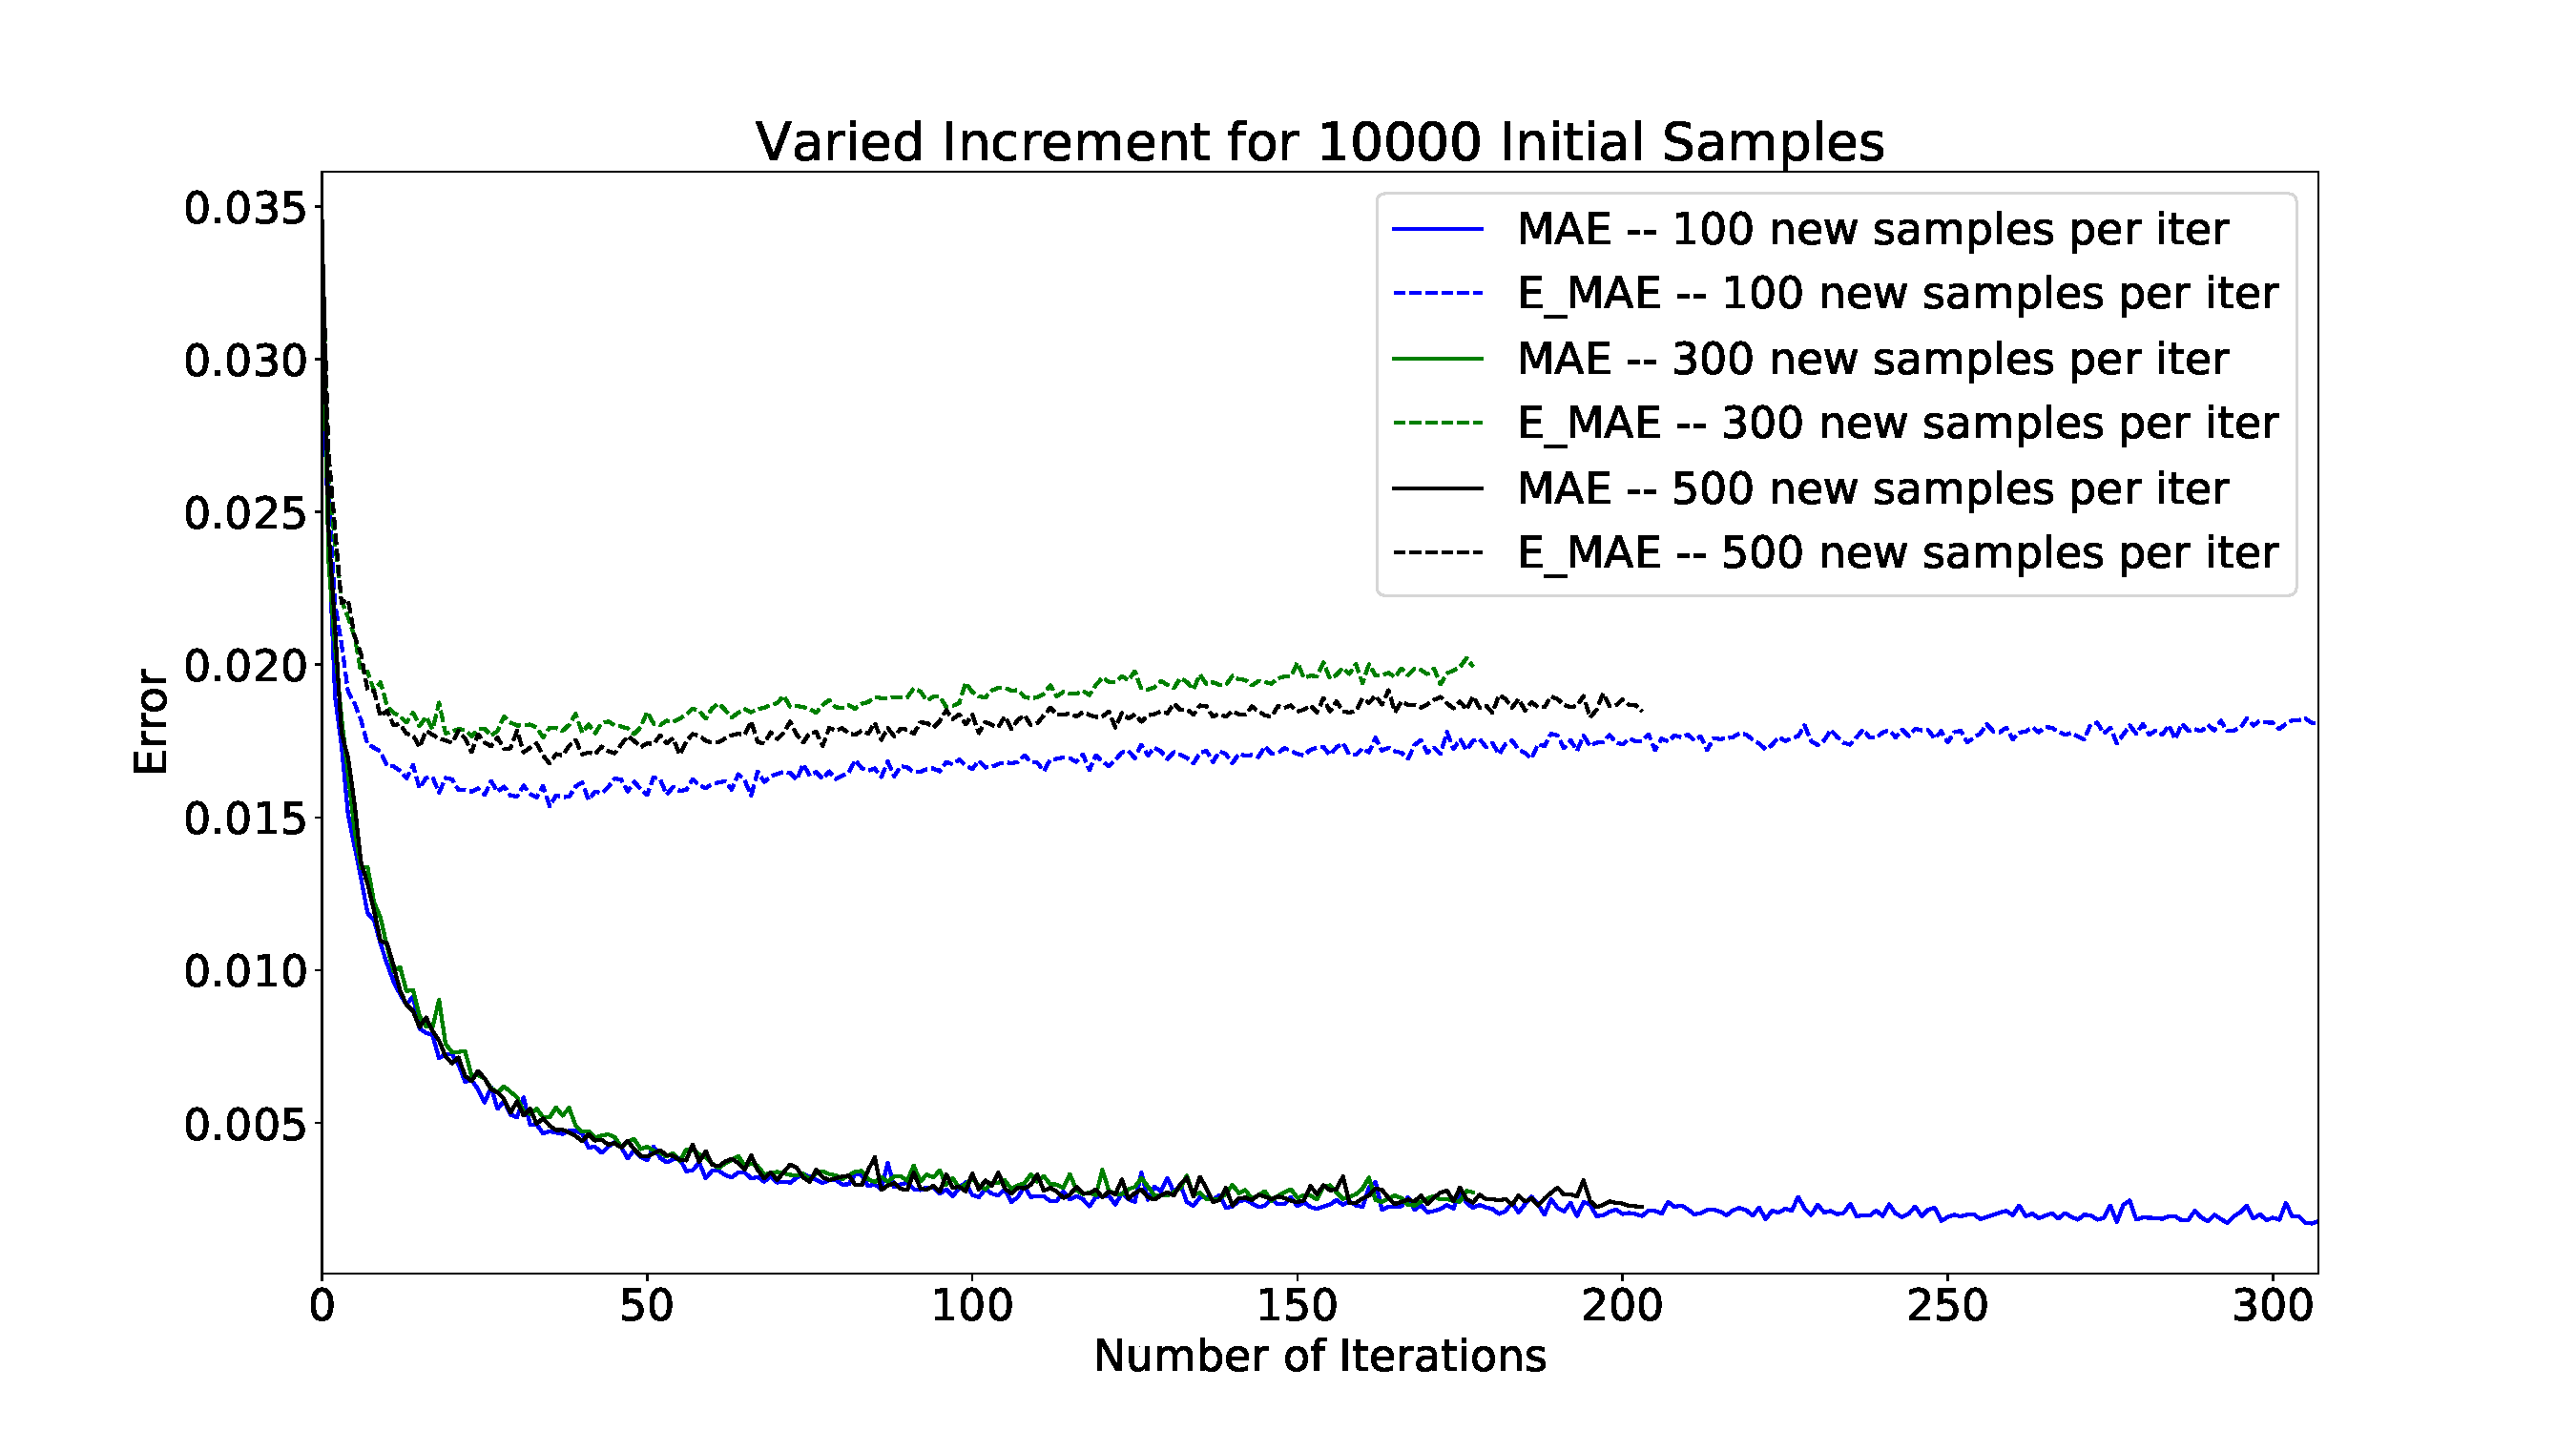
\includegraphics[width=1.1\linewidth]{fig6b_qassincrtime.pdf}
    \end{subfigure}
    \caption{QASS absolute training error over total sample quantity (left) and number of iterations (right). MAE represents surrogate error on the adaptively-sampled training/test set, and E\_MAE on the independent evaluation sets.}
    \label{fig:qassincr}
\end{figure}

The plateau effect in surrogate error on the evaluation set, seen
in~\cref{fig:qassincr}, was universal to all configurations and thought to
warrant further investigation. At first this was suspected to be a residual
effect of retraining the same ANN instance without adjustment to data
normalisation; a "Goldilocks scheme" for checking normalisation drift was
implemented and tested, but did not affect QASS performance. Schemes in which
the ANN is periodically retrained were also discarded, as the retention of
network weights from one iteration to the next was demonstrated to greatly
benefit QASS efficiency. Further insight came from direct comparison between
QASS and a baseline scheme with uniformly random incremental samples, shown
in~\cref{fig:qasssampling}.

\begin{figure}[h]
  \centering
    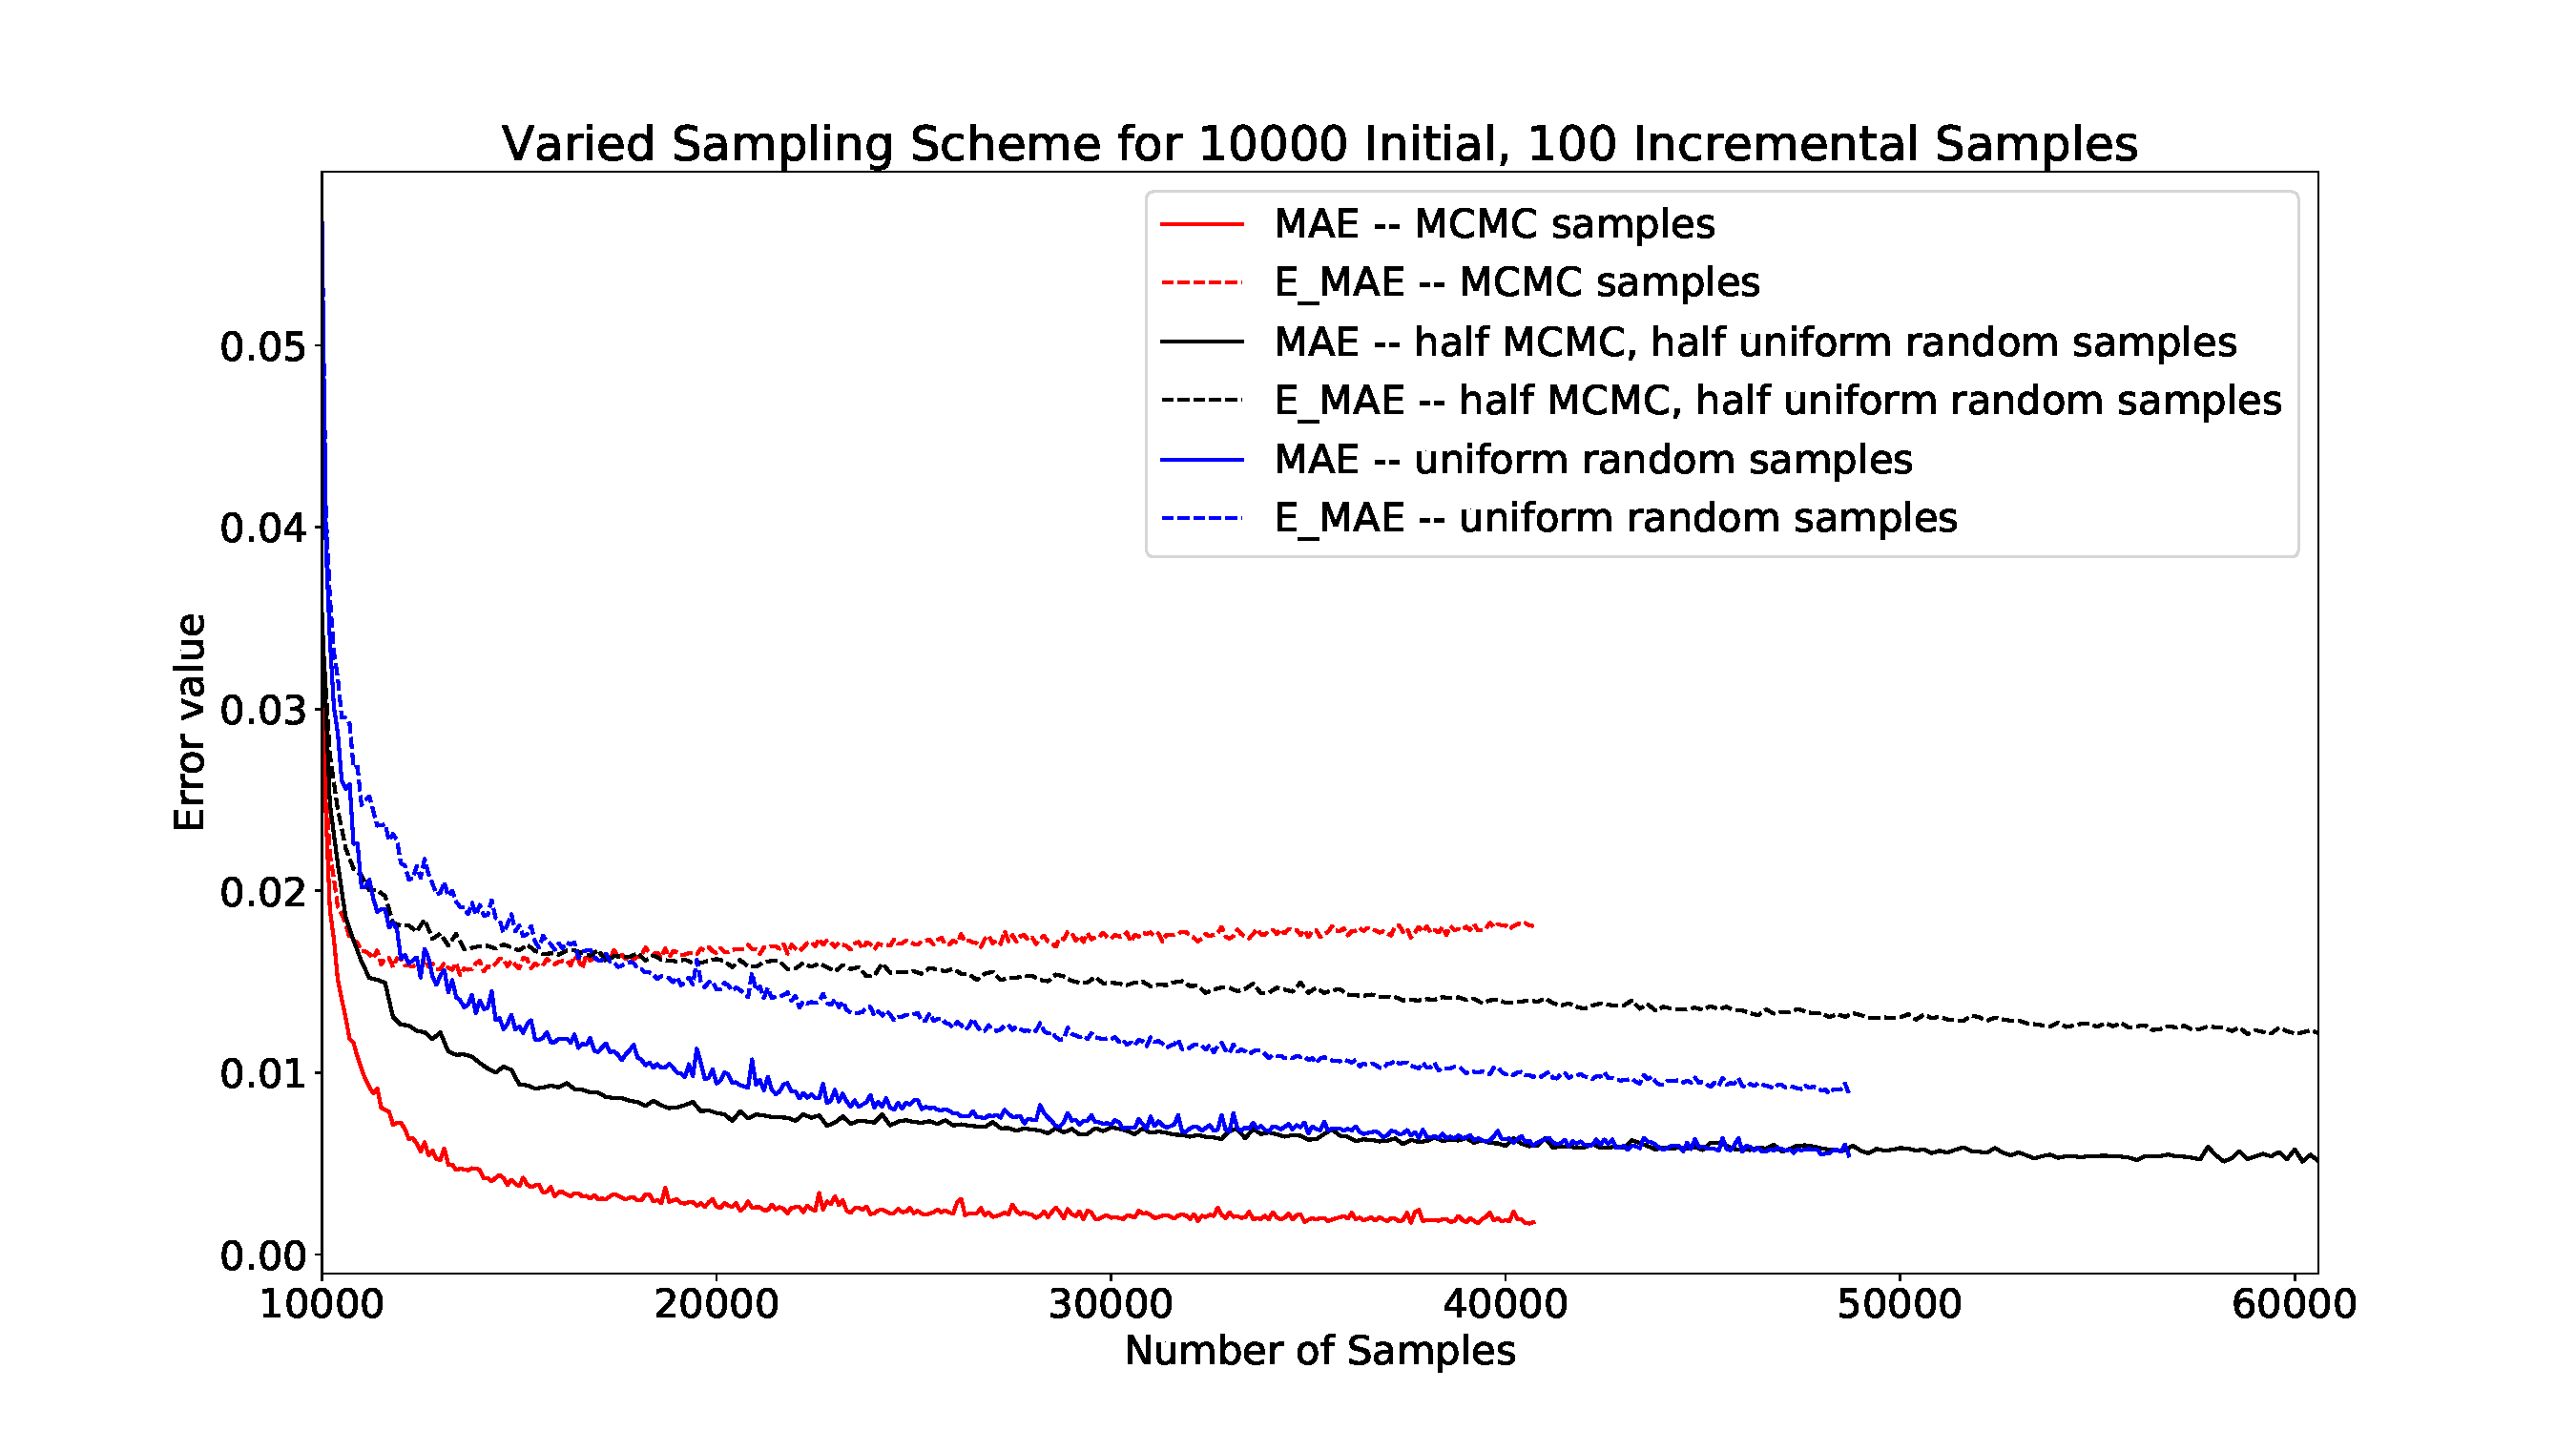
\includegraphics[width=0.8\linewidth]{fig7_qasssampling.pdf}
    \caption{Absolute training error for QASS, baseline scheme, and mixed scheme}
  \label{fig:qasssampling}
\end{figure}

Such tests revealed that while QASS has unmatched performance on its own
adaptively-sampled training set, it is outperformed by the baseline scheme on
uniformly random evaluation sets. We suspected that while QASS excels in
learning the most strongly peaked regions of the TBR theory, this comes at the
expense of precision in broader, smoother regions where uniformly random
sampling suffices. Therefore a mixed scheme was implemented, with half MCMC
samples and half uniformly random samples incremented on each iteration, which
is also shown in~\cref{fig:qasssampling}.
